%The specific components of our system are described in next section.
\label{sec:petra}
%\subsection{Components}

\begin{figure}
\resizebox {0.7\columnwidth} {!} {
\begin{tikzpicture}[x=1.5cm, y=1.5cm, font=\small,
  Component/.style={fill=white, draw, align=center, rounded corners=0.1cm, drop shadow={shadow xshift=0.05cm, shadow yshift=-0.05cm, fill=black}},
  Connection/.style={<->, >=stealth, shorten <=0.05cm, shorten >=0.05cm}]

\foreach \pos/\name in {0/pros1, 0.8/pros2, 1.6/pros3} {
  \node [Component] (\name) at (\pos - 4, \pos) {Prosumer\\(\texttt{RIAPS, geth})};
}

\node [Component] (dso) at (-1, 2.6) {DSO\\(\texttt{RIAPS, geth})};

\fill [fill=black!15] (90:1.5) -- (200:1.5) -- (340:1.5) -- (90:1.5);

\foreach \pos in {90, 200, 340} {
  \node [Component] at (\pos:1.5) {Ethereum\\miner (\texttt{geth})};
}

\node [Component, dotted] (contract) at (0, 0) {Smart contract\\(\texttt{Solidity})};

\draw [Connection, bend left=65] (pros1) to node [midway, left, shift={(-0.25,0)}] {RIAPS ($\emptyset$MQ)} (dso);
\draw [Connection, bend left=55] (pros2) to (dso);
\draw [Connection, bend left=45] (pros3) to (dso);

\draw [Connection, bend right=15] (dso) to (contract);
\draw [Connection, bend right=0] (pros1) to node [midway, below left] {Ethereum} (contract);
\draw [Connection, bend right=0] (pros2) to (contract);
\draw [Connection, bend right=0] (pros3) to (contract);
\end{tikzpicture}

}
\vspace{-0.1in}
\caption{Components of PETra. The DSO and prosumers are comprised of RIAPS components and \texttt{geth} Ethereum clients. The smart contract is implemented in Solidity, a high-level language for Ethereum, and it is executed by a network of \texttt{geth} miners.}
\vspace{-0.1in}
\label{fig:components}
\end{figure}




\begin{figure*} [ht]

\center

\begin{tikzpicture}[x=5.3cm, y=-0.068cm, font=\small,
RedDashed/.style={red, dashed}]
\def\posDSO{0}
\def\posProsumer{1}
\def\posLedger{2}
\def\posOtherProsumer{3}
\foreach \name/\pos in {DSO/\posDSO, Prosumer/\posProsumer, Smart contract/\posLedger, Other prosumer/\posOtherProsumer} {
  \draw (\pos, 0) -- (\pos, 91);
  \node [draw, fill=white, rounded corners=0.1cm] at (\pos, 0) {\name};
}
\newcounter{seqTime}
\setcounter{seqTime}{0}
\foreach \action/\from/\to/\styl/\delta in {
  {withdrawAssets(anonAddress, assets)/\posProsumer/\posDSO/solid/11}, 
  {failedWithdrawal(anonAddress, msg)/\posDSO/\posProsumer/red/8},
  {addEnergyAsset(anonAddress, asset), addFinancialBalance(anonAddress, amount)/\posDSO/\posLedger/solid/8},
  {AssetAdded(anonAddress, assetID, asset)/\posLedger/\posProsumer/dashed/8},
  {postOffer({assetID, price})/\posProsumer/\posLedger/solid/8},
  {OfferPosted({offerID, assetID, price})/\posLedger/\posOtherProsumer/dashed/4},
  {rescindOffer(offerID)/\posProsumer/\posLedger/red/6},
  {OfferRescinded(offerID)/\posLedger/\posOtherProsumer/RedDashed/4},
  {acceptOffer({offerID, assetID})/\posOtherProsumer/\posLedger/solid/8},
  {OfferAccepted({offerID, assetID})/\posLedger/\posProsumer/dashed/4},
  {depositEnergyAsset(assetID), depositFinancial(amount)/\posProsumer/\posLedger/solid/14},
  {AssetDeposited(anonAddress, asset), FinancialDeposited(anonAddress, amount)/\posLedger/\posDSO/dashed/8}%
} {
  \addtocounter{seqTime}{\delta}
  \draw [->, >=stealth, shorten <=0.05cm, shorten >=0.05cm, \styl] (\from, \value{seqTime}) -- (\to, \value{seqTime}) node [midway, above, align=center, text width={abs(\to - \from) * 4.8cm}, fill=white, fill opacity=0.67, text opacity=1] {\footnotesize\texttt{\action}};
}

\end{tikzpicture}
\vspace{-0.2em}
\caption{Sequence diagram of the trading workflow. Solid lines represent RIAPS messages and Ethereum transactions, while dashed lines represent smart-contract events. Messages and transaction in \textcolor{red}{red} stop the trading workflow.}
\label{fig:workflow}
\vspace{-0.12in}
\end{figure*}


Our system contains the following types of components (see Figure~\ref{fig:components} for an illustration):
\begin{itemize}[leftmargin=*]
\setlength{\itemsep}{0pt}%
    \setlength{\topsep}{0pt} 
    \setlength{\partopsep}{0pt}
    \setlength{\parsep}{0pt}
    \setlength{\parskip}{0pt}%
\item DSO: There is a single component of this type, which represents the Distribution System Operator of the microgrid. 
The primary responsibilities of this component are ensuring the safe operation of the microgrid and regulating the total load of the microgrid.
To this end, the DSO component can limit the energy and financial assets that the prosumers' withdraw for trading, and it can also set a price policy for the microgrid.
Note that this component does not have to be online during trading, so the reliability of the system does not hinge on the reliability of this component.
\item Prosumer: There is a component of this type for every household.
The prosumer components are responsible for trading energy production and consumption for their households.
To do so, a component first estimates the future production and consumption of the household, withdraws energy production or consumption assets from the DSO, and then trades these assets with other prosumers.
To ensure that trading does not compromise the household's privacy, the component uses randomly generated anonymous addresses for trading, which hide the identities of trade partners from each other.
\item Smart contract: 
%There is a single component of this type, which is deployed as an Ethereum contract on the private blockchain. 
This component (deployed as an Ethereum contract on the private blockchain) is responsible for keeping track of the energy and financial assets belonging to each anonymous address, enabling prosumers to post trade offers, and exchanging assets when another prosumer decides to take an offer.
The contract is executed in a decentralized manner by a network of miners, which provides reliability. Additionally, we have several Ethereum clients, one per prosumer and one for the DSO, which interact with the smart contract.
\end{itemize}

\vspace{-0.08in}
\subsection{Assets and Data Structures}

The ability to specify points or intervals in time is crucial.  For
example, control signals specify how the microgrid load should change
at certain points in time, energy trades specify when energy will be
consumed or produced, etc.  To facilitate representing signals and
transactions, we divide time into fixed-length intervals, and specify
points or periods in time using these discrete timesteps.  The length
of the time interval is determined based on the timing assumptions of
the physical power system.  For example, the
time interval may as low as 4 seconds, which corresponds to how frequently
the control signal of the DSO typically changes \cite{federal2011frequency}.

Prosumers trade energy production and consumption with each other, which are represented in PETra by energy assets, which is a structure that comprises the following fields: (a)
 \texttt{int64 power}: non-negative amount of power to be produced or consumed (for example, measured in watts), (b)
 \texttt{uint64 start}: first time interval in which energy is to be produced (or consumed), and (c) \texttt{uint64 end}: last time interval in which energy is to be produced (or consumed).
An asset with positive power value represents energy production, and we call it an \texttt{EnergyProductionAsset}.
An asset with negative power value, on the other hand, represents energy consumption, and we call it an \texttt{EnergyConsumptionAsset}.

Energy trading must also involve the transfer of currencies, which are represented by financial assets.
A \texttt{FinancialAsset} is simply an \texttt{uint64} value, denominated in a fiat currency.


%\vspace{-0.08in}
\subsection{Trading Workflow}

Next, we discuss the trading workflow that is used by prosumers to trade energy production and consumption assets, as well as financial assets with each other.
This workflow involves both off-blockchain messaging (using RIAPS), and on-blockchain transactions and events.
We list these messages, transactions, and events in the order in which they typically appear in the workflow.
Figure~\ref{fig:workflow} shows a graphical illustration of the workflow.
\vspace{-0.1em}
\begin{itemize}[leftmargin=*]
\setlength{\itemsep}{0pt}%
    \setlength{\topsep}{0pt} 
    \setlength{\partopsep}{0pt}
    \setlength{\parsep}{0pt}
    \setlength{\parskip}{0pt}%
\item 
\texttt{withdrawAssets(anonAddress, assets)}: RIAPS message sent by a prosumer to the DSO, asking the DSO to transfer energy and/or financial assets from the prosumer's account at the DSO to an anonymous address to protect her privacy.
Before sending this message, the prosumer should generate a new random anonymous address.
The message specifies the assets that the prosumer wishes to withdraw, and the anonymous address to which the DSO should transfer them, which must be cryptographically signed by the prosumer.
Note that the prosumer may send this message long before actually engaging in trading, so the DSO does not have to be online continuously.
\item \texttt{failedWithdrawal(anonAddress, msg)}: RIAPS message sent by the DSO to the prosumer,
notifying the prosumer that the requested assets cannot be withdrawn due to, e.g., energy safety requirements or insufficient funds.
\item \texttt{addEnergyAsset(anonAddress, asset)},\\\texttt{addFinancialBalance(anonAddress, amount)}:
smart contract transaction called by the DSO, creating energy and financial assets on the blockchain and transferring them to an anonymous address.
Before recording this transaction, the DSO must first verify whether enabling the prosumer to trade these assets would violate any safety requirements.
The transaction specifies the assets and the anonymous address to which they are transferred, and it must be cryptographically signed by the DSO.
\item \texttt{AssetAdded(anonAddress, assetID, asset)},\\\texttt{FinancialAdded(anonAddress, amount)}: events broadcast by the smart contract,
notifying the prosumer that the requested assets have been transferred to the anonymous address.
\item \texttt{postOffer(assetID, price)}: smart contract transaction called by a prosumer, publicly posting an energy bid or ask.
If the prosumer is interested in buying energy, then it posts an energy bid, which specifies an energy consumption asset and a price.
If the prosumer is interested in selling, then it posts an energy ask, which specifies an energy production asset and a price.
vIn both cases, the transaction must be cryptographically signed by the private key of the address, and it locks the assets until the offer is accepted or rescinded.
\item \texttt{OfferPosted(offerID, assetID, price)}:
event broadcast by the smart contract, notifying prosumers that an offer was posted.
\item \texttt{rescindOffer(offerID)}:
smart contract transaction called by a prosumer, rescinding an offer.
The transaction must be cryptographically signed by the private key of the poster.
\item \texttt{acceptOffer(offerID, assetID)}:
smart contract transaction called by a prosumer,
accepting a previously posted offer. % and transferring the assets between the prosumers.
If the offer was an energy bid, then the other prosumer has to provide an energy production assets;
if the offer was an energy ask, then the other prosumer has to provide both energy consumption and financial assets.
In both cases, the transaction must be cryptographically signed by the private key of the other prosumer's anonymous address.
If there is an overlap between the time intervals of the offered asset, and the asset provided by the other prosumer, then the intersecting parts of the assets are exchanged and the non-overlapping parts are returned to their original owners.
Similarly, based on the price and exchanged energy assets, a part of the financial asset is transferred to the seller, while the rest is returned to the seller. 
%If the energy assets match each other, and the financial asset matches the price, then the assets are exchanged between the prosumers' anonymous addresses. 
\item \texttt{OfferAccepted(offerID, assetID)}:
event broadcast by the smart contract,
notifying the prosumer that its offer has been accepted, and the assets have been exchanged.
\item \texttt{depositEnergyAsset(assetID)},\\\texttt{depositFinancial(amount)}:
smart contract transactions called by a prosumer,
depositing energy and financial assets to the prosumer's account.
The transaction specifies the assets, and it must be cryptographically signed by the anonymous address that owns them.
Note that to protect privacy, the transaction does not specify the prosumer, so the DSO has to keep track of which prosumer has used which anonymous address.
\item \texttt{AssetDeposited(anonAddress, assetID)},\\\texttt{FinancialDeposited(anonAddress, amount)}:
event broadcast by the smart contract,
notifying the DSO that assets have been deposited from anonymous address, which triggers the transfer of these assets to the prosumer's account at the DSO.
\end{itemize}

\begin{comment}
\begin{figure}
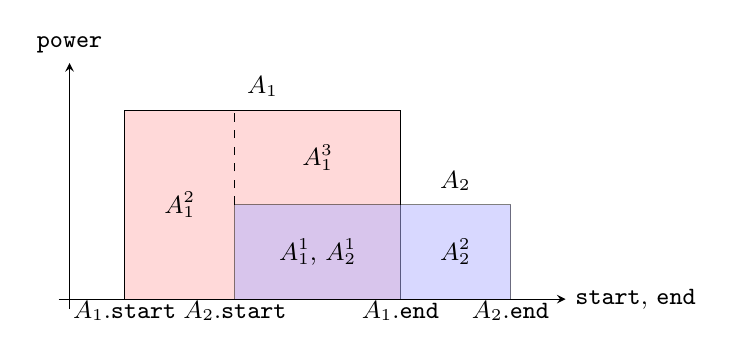
\begin{tikzpicture}[x=0.7cm,y=0.3cm, font=\small]
\draw [->, >=stealth] (-0.2,0) -- (9,0) node [right] {\texttt{start}, \texttt{end}};
\draw [->, >=stealth] (0,-0.4) -- (0,10) node [above] {\texttt{power}};

\draw [fill=red!15] (1, 0) -- (1, 8) -- (6, 8) -- (6, 0);
\draw [fill=blue!30, opacity=0.5] (3, 0) -- (3, 4) -- (8, 4) -- (8, 0);

\node at (3.5, 9) {$A_1$};
\node at (7, 5) {$A_2$};

\node at (2, 4) {$A_1^2$};
\node at (4.5, 6) {$A_1^3$};
\node at (4.5, 2) {$A_1^1$, $A_2^1$};
\node at (7, 2) {$A_2^2$};

\node at (1, -0.5) {$A_1$.\texttt{start}};
\node at (6, -0.5) {$A_1$.\texttt{end}};
\node at (3, -0.5) {$A_2$.\texttt{start}};
\node at (8, -0.5) {$A_2$.\texttt{end}};

\draw [dashed] (3,4) -- (3,8);
\end{tikzpicture}
\caption{Example of exchanging two assets, $A_1$ and $A_2$, that do not match each other perfectly.
First, asset $A_1$ is divided into three smaller assets $A_1^1$, $A_1^2$, and $A_1^3$, while asset $A_2$ is divided into two smaller assets $A_2^1$ and $A_2^2$.}
\label{fig:assetExchange}
\end{figure}
\end{comment}

\subsection{Case Study}
\label{sec:results}

\definecolor{blueLine}{RGB}{57,106,177}
\definecolor{blueFill}{RGB}{114,147,203}
\definecolor{redLine}{RGB}{204,37,41}

\begin{figure}[t]
\centering
% \vspace{-0.1in}
%    \makebox[\linewidth]{
       % 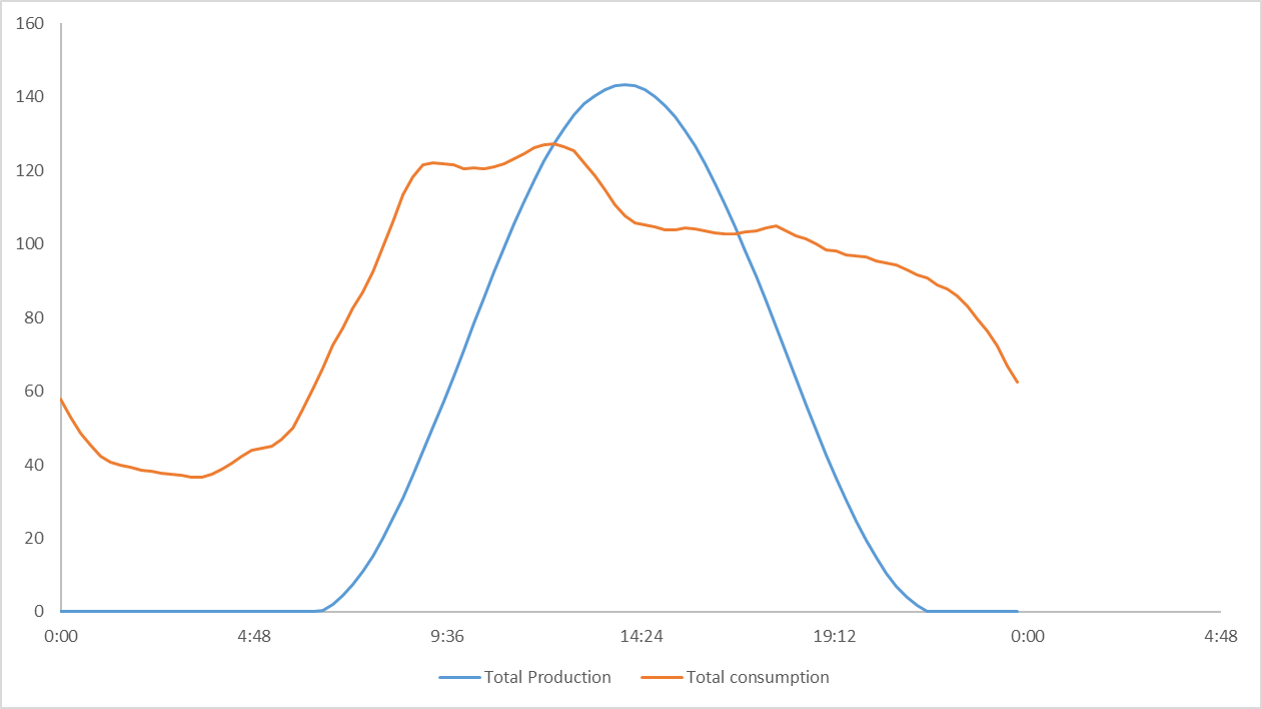
\includegraphics[width=1.0\linewidth]{loadprofile.png}
%    }

\begin{tikzpicture}
\begin{axis}[
  font=\small,
  width=1.05\columnwidth,
  height=0.61\columnwidth,
  ymin=-1,
  ymax=200,
  xmin=-1,
  xmax=97,
  legend pos=north west,
  xlabel=Time,
  ylabel={[kWh]},
  ytick={0, 50, 100, 150},
  xtick={0, 32, 64, 95},
  xticklabels={0:00, 8:00, 16:00,  23:45},
%  ymajorgrids,
%  xmajorgrids,
]
\addplot[no markers, solid, blueLine, semithick] table[x expr=\coordindex, y=Production, comment chars={\%}] {total_prod_cons.csv};
\addlegendentry{Total production};
\addplot[no markers, solid, redLine, semithick] table[x expr=\coordindex, y=Consumption, comment chars={\%}] {total_prod_cons.csv};
\addlegendentry{Total consumption};
\end{axis}
\end{tikzpicture}
\vspace{-2em}
\caption{Load profile and Generation Profile in KWH per 15 minute interval. The horizontal axis shows time of day.}
\label{fig:profile}
% \vspace{-0.2in}
\end{figure}

We use  data collected by Siemens, from a microgrid in Germany,  to demonstrate a simulated transactive scenario. Figure \ref{fig:profile} shows the total energy produced in this system over the day, and  the total energy consumed. We use a $T=15$ minute time interval for bids and asks. We picked a 3.5 hour time interval (from 2:15pm to 5:45pm) and 2 producers and 7 consumers that overlapped with the peak of production capacity (see Figure \ref{fig:profile}). We ran the network across six virtual machines, each with 2 virtual CPUs, 4 GB RAM and 40 GB hard-disk. The \texttt{geth} clients (one per actor) and miners were equally distributed on this network. The actors (Prosumers and DSO) were written in Python, and they communicated with the \texttt{geth} clients using JSON-RPC API provided by Ethereum. The  actors communicated with each other using RIAPS and polled the blockchain ledger for transactional updates using custom filters, which are supported by the Ethereum API.
%\Aron{We could claim that we picked this time interval because it was the busiest.}}} The system has $2$  producers and 7 consumers from a microgrid installation in Germany.  
%\Abhishek{Mike - please explain the figures. they both look very similar.}

Figure~\ref{fig:offer_histogram} shows the distribution of the time between when an offer was made by a producer, and then the time when the offer was accepted by a consumer and cleared. As shown by Figure~\ref{fig:workflow}, this includes two transactions, \texttt{postOffer} and \texttt{acceptOffer}, which have to be verified and recorded by the miners. To clear these two transactions, at least two blocks need to be mined. The statistics of the clearing-time distribution are as follows: 
average = 11.79 seconds, median = 11 seconds, variance = 46.74, maximum = 38 seconds, minimum = 0 seconds, and 90\% of trades were cleared within 23 seconds or less.

%Figure \ref{} shows the setup of virtual machines on which we play out the simulated transactions capturing the timing restrictions and showing the feasibility of the system, while maintaining the safety constraints and the privacy restrictions. 


\begin{figure}[t]
% \vspace{-0.1in}
%    \makebox[\linewidth]{
       % 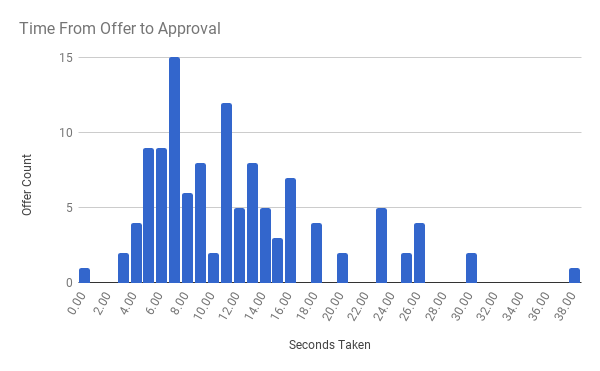
\includegraphics[width=1.0\linewidth]{offer_histogram.png}
%        }
  \begin{tikzpicture}
\begin{axis}[
  font=\small,
  width=1.05\columnwidth,
  height=0.54\columnwidth,
  ymin=0,
  ymax=16,
  xmin=-0.5,
  xmax=38.5,
  xlabel={Time until offer was accepted [seconds]},
  ylabel={Number of offers},
  ymajorgrids,
]
\addplot[ybar, bar width=3pt, no markers, fill=blueFill, draw=blueLine, semithick] table[x=Seconds, y=Count, comment chars={\%}, col sep=comma] {TimePerOfferHistogram.csv};
\end{axis}
\end{tikzpicture}
\vspace{-1em}
\caption{Histogram of time it takes to clear the two transactions related to post offer and accept offer. 90\% of the trades were closed within 23 seconds or less.}
\label{fig:offer_histogram}
% \vspace{-0.2in}
\end{figure}



\subsection{Requirements Analysis Discussion}
 \label{sec:discussion} 
We conclude this section with a brief discussion of how PETra satisfies the requirements outlined in Section~\ref{sec:requirements}.

\textbf{Communication Fabric:}
%\Aron{Abhishek, could you please check if the statements about RIAPS are correct?}
%\Abhishek{I made minor edits}
The key requirements for communication are reliability and security. 
In PETra, communication and messaging services are built on (a) RIAPS between the DSO and prosumers, and (b) blockchain transactions and events between the smart contract and other components.
The RIAPS communication layer \cite{eisele2017riaps} presents a reliable messaging service, which  is being currently extended to provide message confidentiality, integrity, and non-repudiation with the help of digital signatures.
Since communication between prosumers and the DSO (i.e. withdrawal) may happen well in advance of actual trading, the DSO and the messaging service do not have to be online continuously.
Combined with the features of RIAPS, this flexibility in uptime leads to a very high level of reliability. 

For messaging between the smart contract and other components, the blockchain provides a secure and reliable communication medium.
The  blockchain ledger is an immutable, complete, and fully auditable record, which guarantees integrity and non-repudiation for transactions and events.
Note that---by design---the blockchain does not provide confidentiality, since every transaction and event is public; we will discuss privacy implications and requirements in detail below.
Finally, the blockchain provides a high level of reliability since the ledger is maintained by multiple nodes, which can reach consensus even in the presence of some misbehaving or malicious nodes.

\textbf{Operational Safety, Cyber-Physical Security, and Market Safety:}
For safety and cyber-physical security, it is crucial to ensure that  trading activity cannot compromise the stability of the grid and congestion constraints are respected.
PETra achieves these goals by enabling the DSO to tightly control the amount of energy that a prosumer may (offer to) sell or buy.
A prosumer's energy trading workflow (see Figure~\ref{fig:workflow}) always begins with a withdrawal from the DSO.
By limiting the amount assets that can be withdrawn, the DSO limits the bids and asks that may be posted by a prosumer, thereby enforcing safety requirements (e.g., preventing a prosumer from offering to produce more power than her production capacity).
Fine-grained withdrawal rules based on time, power, etc, can be used to prevent a wide range of negligent or malicious trading.

To protect the prosumers' interests, 
we must enable them to detect and prove if they are incorrectly billed or denied fair participation in the market.
%we must ensure that incorrect billing and unfair participation can be detected and proved. we must ensure that billing is correct correctness of billing and fairness of the trading system.
PETra meets these goals due to the public, fully auditable, and immutable nature of the blockchain ledger.

\textbf{Privacy:}
Privacy requirements dictate that prosumers cannot gain information regarding other prosumers' consumption and production---not even if they are trade partners.
This requirement presents an interesting challenge since every transaction on the blockchain ledger is public.
PETra provides privacy through pseudonymous trading; instead of real identities, prosumers use randomly chosen addresses for trading with each other.
However, pseudonymous addresses could be de-anonymized either by (a) learning which addresses belong to the same prosumer or (b) using the prosumers' communication addresses (e.g., IP addresses used to send transactions).
%There are two threats to privacy: de-anonymization by linking addresses together and by linking addresses to communication addresses (e.g., IP addresses)
Firstly, by employing a large number of anonymous addresses, a prosumer can effectively prevent de-anonymization attacks that would link her addresses together.\footnote{Note that generating new addresses is trivial.} %, prosumers can prevent attacks that could de-anonymize trading by linking addresses together
Secondly, by combining our platform with a communication anonymity solution, such as onion routing, we can prevent de-anonymization based on communication addresses.

%for communication anonymity (e.g., onion routing, such as Tor), we can prevent de-anonymization using network traffic analysis


%\subsection{Privacy Protection}

%By combining our platform with a communication anonymity solution, such as onion routing, we can provide pseudonymous trading service, in which there is no apparent connection between the addresses used for trading and the prosumers owning them.


